% SPDX-FileCopyrightText: 2026 Niels Bonde Jensen
% SPDX-License-Identifier: MIT
% Carve-out: the code in this file is MIT-licensed. The cover copy embedded in it ---
% headline, blurb, pull quote, reader line, biography --- is part of the book text,
% (c) 2026 Niels Bonde Jensen, all rights reserved.
% cover_wrap.tex --- KDP full-wrap builder for The Billiard Ball Universe (Concept A: The Engraved Plate)
% ONE number to update at the end: \PAGECOUNT. Flip \ARTFINALtrue when cover_recursive_ball.png exists.
\documentclass{article}
\usepackage{calc}
\newcommand\PAGECOUNT{202}                                   % FINAL. Interior declared final 2026-08-21; both editions 202 pp, 0/0.
% CREAM stock, ruled 2026-08-20 (was 0.002252in = KDP white, an inherited default
% rather than a decision). KDP: white 0.002252 in/page, cream 0.0025 in/page.
% At the final 202 pp this is 0.5050in, not 0.4549in -- 0.05in apart, so the
% constant and \PAGECOUNT must be right together or the wrap is wrong twice over.
\newlength\spinew \setlength\spinew{0.0025in * \real{\PAGECOUNT}}    % KDP cream paper
\newlength\bleed  \setlength\bleed{0.125in}
\newlength\wrapw  \setlength\wrapw{12in + \spinew + 2\bleed}
\newlength\wraph  \setlength\wraph{9in + 2\bleed}
\usepackage[paperwidth=\wrapw,paperheight=\wraph,margin=0pt]{geometry}
\usepackage[T1]{fontenc}
\IfFileExists{tgpagella.sty}{\usepackage{tgpagella}}{\usepackage{mathpazo}}
\usepackage{microtype,tikz,graphicx,xcolor}
% Sanguine plate, 2026-08-20: the ground moved one step off paper-white and the
% plate is pulled in red ink. Paper plus one printer's ink -- the drawing is the
% same drawing. See cover/gen_sanguine.py for the ramp and why it is a tritone.
\definecolor{ivory}{HTML}{EDE4CE}\definecolor{ink}{HTML}{1A1A1A}\definecolor{oxblood}{HTML}{6B2E2E}
\newif\ifARTFINAL \ARTFINALtrue
\newif\ifOXRULE   \OXRULEtrue
\newcommand\ARTW{3.7in}   % art width; SQUARE source per brief (portrait source would overflow the front)
% EAN-13 for our own ISBN 978-87-977519-1-6. Generated (see the file's header);
% we print the barcode ourselves rather than let KDP overlay one, because KDP's
% overlay carries KDP's free ISBN, which is Amazon-locked and would split the
% edition Phase 2 needs to keep whole.
% ean13.tex --- EAN-13 for ISBN 978-87-977519-1-6, generated, do not hand-edit.
% Pattern computed from the EAN-13 spec and decoded back to 9788797751916 before
% emission; regenerate with cover/gen_ean13.py if the ISBN ever changes,
% and verify the built cover with cover/scan_ean13.py.
% \EANthirteen{x}{y}: bottom-left of the LEFT QUIET ZONE at (x,y), units of
% the enclosing tikzpicture (x=1in,y=1in). Symbol is 1.3213 x 0.8681 in at 90% mag.
\newcommand{\EANthirteen}[2]{%
  \begin{scope}[shift={(#1,#2)}]
    %% quiet zones: the symbol must sit on unbroken white
    \fill[white] (-0.04000,-0.11500) rectangle (1.36130,1.02311);
    \fill[black] (0.12862,0.00000) rectangle (0.14031,0.86811);
    \fill[black] (0.15201,0.00000) rectangle (0.16370,0.86811);
    \fill[black] (0.17539,0.05846) rectangle (0.21047,0.86811);
    \fill[black] (0.22217,0.05846) rectangle (0.24555,0.86811);
    \fill[black] (0.28063,0.05846) rectangle (0.29232,0.86811);
    \fill[black] (0.31571,0.05846) rectangle (0.32740,0.86811);
    \fill[black] (0.36248,0.05846) rectangle (0.37417,0.86811);
    \fill[black] (0.39756,0.05846) rectangle (0.40925,0.86811);
    \fill[black] (0.42094,0.05846) rectangle (0.45602,0.86811);
    \fill[black] (0.46772,0.05846) rectangle (0.49110,0.86811);
    \fill[black] (0.51449,0.05846) rectangle (0.52618,0.86811);
    \fill[black] (0.53787,0.05846) rectangle (0.57295,0.86811);
    \fill[black] (0.58465,0.05846) rectangle (0.61972,0.86811);
    \fill[black] (0.63142,0.05846) rectangle (0.65480,0.86811);
    \fill[black] (0.66650,0.00000) rectangle (0.67819,0.86811);
    \fill[black] (0.68988,0.00000) rectangle (0.70157,0.86811);
    \fill[black] (0.71327,0.05846) rectangle (0.72496,0.86811);
    \fill[black] (0.76004,0.05846) rectangle (0.77173,0.86811);
    \fill[black] (0.79512,0.05846) rectangle (0.80681,0.86811);
    \fill[black] (0.83020,0.05846) rectangle (0.86528,0.86811);
    \fill[black] (0.87697,0.05846) rectangle (0.90035,0.86811);
    \fill[black] (0.92374,0.05846) rectangle (0.94713,0.86811);
    \fill[black] (0.95882,0.05846) rectangle (0.99390,0.86811);
    \fill[black] (1.00559,0.05846) rectangle (1.01728,0.86811);
    \fill[black] (1.04067,0.05846) rectangle (1.06406,0.86811);
    \fill[black] (1.08744,0.05846) rectangle (1.11083,0.86811);
    \fill[black] (1.12252,0.05846) rectangle (1.13421,0.86811);
    \fill[black] (1.14591,0.05846) rectangle (1.15760,0.86811);
    \fill[black] (1.20437,0.00000) rectangle (1.21606,0.86811);
    \fill[black] (1.22776,0.00000) rectangle (1.23945,0.86811);
    %% human-readable: leading digit in the left quiet zone, groups of six
    \node[anchor=base east,inner sep=0pt,black] at (0.12278,-0.00800) {\sffamily\fontsize{7}{7}\selectfont 9};
    \node[anchor=base,inner sep=0pt,black] at (0.40925,-0.00800) {\sffamily\fontsize{7}{7}\selectfont\textls[110]{788797}};
    \node[anchor=base,inner sep=0pt,black] at (0.95882,-0.00800) {\sffamily\fontsize{7}{7}\selectfont\textls[110]{751916}};
    %% the registry wants the ISBN itself readable, not only the EAN digits
    \node[anchor=south,inner sep=0pt,black] at (0.66065,0.90311) {\sffamily\fontsize{7.5}{8}\selectfont\textls[60]{ISBN 978-87-977519-1-6}};
  \end{scope}}

\pagestyle{empty}
\begin{document}\color{ink}
\begin{tikzpicture}[remember picture,overlay,shift={(current page.south west)},x=1in,y=1in]
  \fill[ivory] (0,0) rectangle (\wrapw,\wraph);
  % panel trim coordinates (inches): back [0.125,6.125], spine, front [6.125+s, 12.125+s]
  \pgfmathsetmacro\s{\spinew/1in}
  \pgfmathsetmacro\fL{6.125+\s}      % front trim left
  \pgfmathsetmacro\fC{\fL+3.0}       % front centerline
  % ---- double frames, inset 0.28in from trim ----
  \foreach \a/\b in {0.6/1.6}{}
  \draw[ink,line width=1.6pt] (0.125+0.28,0.125+0.28) rectangle (6.125-0.28,9.125-0.28);
  \draw[ink,line width=0.6pt] (0.125+0.28+0.055,0.125+0.28+0.055) rectangle (6.125-0.28-0.055,9.125-0.28-0.055);
  \draw[ink,line width=1.6pt] (\fL+0.28,0.125+0.28) rectangle (\fL+6-0.28,9.125-0.28);
  \draw[ink,line width=0.6pt] (\fL+0.28+0.055,0.125+0.28+0.055) rectangle (\fL+6-0.28-0.055,9.125-0.28-0.055);
  % ================= FRONT =================
  % Title is a three-line stack: the long line "BILLIARD BALL" is 473pt at 60pt --- far wider
  % than the ~393pt inner panel --- so it is set at 46pt (362pt) and "THE" rides as a kicker.
  \node[anchor=north] at (\fC,9.125-0.58) {\fontsize{13}{15}\selectfont\textls[180]{NO MAGIC ANYWHERE}};
  \node[anchor=north] at (\fC,9.125-1.05) {\fontsize{26}{28}\bfseries\selectfont\textls[120]{THE}};
  \node[anchor=north] at (\fC,9.125-1.55) {\fontsize{46}{48}\bfseries\selectfont BILLIARD BALL};
  \node[anchor=north] at (\fC,9.125-2.25) {\fontsize{46}{48}\bfseries\selectfont UNIVERSE};
  % 1.8pt, not 1.1: at 90px a 1.1pt rule is invisible, so the only note of
  % colour on the thumbnail was doing no work at all.
  \ifOXRULE \draw[oxblood,line width=1.8pt] (\fC-1.55,9.125-3.05) -- (\fC+1.55,9.125-3.05);
  \else     \draw[ink,line width=0.6pt]     (\fC-1.55,9.125-3.05) -- (\fC+1.55,9.125-3.05); \fi
  % art band, centered; square \ARTW x \ARTW
  \pgfmathsetmacro\artw{3.7}
  \ifARTFINAL
    \node[anchor=north] at (\fC,9.125-3.17) {\includegraphics[width=\ARTW]{cover_recursive_ball_sanguine}};
  \else
    \draw[ink,line width=0.6pt] (\fC-\artw/2,9.125-3.28-\artw) rectangle (\fC+\artw/2,9.125-3.28);
    \draw[ink,line width=0.4pt] (\fC-\artw/2,9.125-3.28-\artw) -- (\fC+\artw/2,9.125-3.28);
    \draw[ink,line width=0.4pt] (\fC-\artw/2,9.125-3.28) -- (\fC+\artw/2,9.125-3.28-\artw);
    \node at (\fC,9.125-3.28-\artw/2) {\small cover\_recursive\_ball --- placeholder (square, per brief)};
  \fi
  \node[anchor=north] at (\fC,9.125-7.32) {\fontsize{24}{26}\itshape\selectfont A World With No Bottom};
  \node[anchor=south] at (\fC,0.125+0.60) {\fontsize{18}{20}\selectfont\textls[120]{NIELS BONDE JENSEN}};
  % ================= SPINE =================
  \node[rotate=-90,anchor=center] at (6.125+\s/2,9.125-2.55) {\fontsize{11.5}{13}\selectfont\textls[60]{THE BILLIARD BALL UNIVERSE}};
  \node[rotate=-90,anchor=center] at (6.125+\s/2,0.125+2.05) {\fontsize{11.5}{13}\selectfont\textls[60]{NIELS BONDE JENSEN}};
  \fill[ink] (6.125+\s/2,4.625) circle (0.055); \draw[ivory,line width=0.5pt] (6.125+\s/2,4.625)++(-0.02,0.03) arc (130:310:0.036);
  % ================= BACK =================
  \node[anchor=north west,text width=4.6in,align=left] at (0.125+0.62,9.125-0.72) {%
    {\fontsize{15}{18}\bfseries\selectfont\hyphenpenalty=10000\exhyphenpenalty=10000 A universe with no bottom --- argued\\ by an author who shows you where he loses.\par}\vspace{9pt}
    {\fontsize{10.5}{14.5}\selectfont
    As a child, Niels Bonde Jensen decided that two things were cheating: forces that pull across empty space, and borders that end the questions. This book is the adult case for the universe the child demanded --- infinitely layered, everything pushing, everything made of something smaller, without end.\par\vspace{5.5pt}
    It is not a book that claims victory. Its central argument was fought out, round by round, against an artificial mind armed with the strongest objections in the written tradition --- and the concessions, in both directions, are kept on the page. Its physics chapter grades its own wounds: the three-hundred-year-old pincer of drag and heat; the gravitational waves of LIGO; Bell's theorem, aimed at the book's first sentence by name. Where the toy universe breaks, the breaks are shown --- in a table, which the book then reads backward, as a specification of the layer below.\par\vspace{5.5pt}
    What survives is smaller and harder than what the author walked in with: not proof, but a universe with exactly one mystery --- why there is anything at all --- and no magic anywhere else. Along the way: why an infinite universe contains other yous; why that is comforting rather than crushing; why your responsibility is the local surplus of joy over suffering; and why, globally, nothing is special --- while locally, you are.\par}\vspace{8pt}
    \begin{center}\begin{minipage}{3.7in}\centering
      \rule{3.1in}{0.5pt}\\[5pt]
      {\fontsize{13}{16}\itshape\selectfont ``Globally nothing is special.\\ Locally, you are. Live there.''}\\[5pt]
      \rule{3.1in}{0.5pt}
    \end{minipage}\end{center}\vspace{8pt}
    % Bottom two lines constrained to 2.9in so they clear the KDP barcode reserve
    % (box left edge x=3.775in; text left edge x=0.745in -> 0.745+2.9=3.645 < 3.775).
    \noindent\parbox{2.9in}{%
      {\fontsize{9}{12}\selectfont For physicists, and for the interested layman: footnotes decode every term, a dictionary and a primer wait in the appendices, and nothing essential hides outside the plain prose.\par}\vspace{6pt}
      {\fontsize{9}{12}\itshape\selectfont Niels Bonde Jensen is a Danish software engineer. He has believed the universe has no bottom since before he could say why.\par}}};
  % Barcode. The reserve stays 2.0 x 1.2in at 0.35in from the trim edges (KDP's
  % requirement); the symbol sits centred inside it. Bottom of the back panel,
  % nearest the spine, per DBC's own instruction ("nederst naermest ryggen").
  \fill[white] (6.125-0.35-2.0,0.125+0.35) rectangle (6.125-0.35,0.125+0.35+1.2); % barcode reserve
  \EANthirteen{4.1144}{0.621}
\end{tikzpicture}
\end{document}
